\documentclass[12pt,a4paper]{article}
% chktex-file 36

% Encoding and language
\usepackage[utf8]{inputenc}
\usepackage[T1]{fontenc}
\usepackage[english]{babel}

% Layout and spacing
\usepackage[margin=2.5cm]{geometry}
\usepackage{setspace}
\usepackage{titlesec}

% Graphics and tables
\usepackage{graphicx}

% Lists and formatting
\usepackage{enumitem}
\usepackage{fancyhdr}
\usepackage{lastpage}

% Hyperlinks
\usepackage{hyperref}

\hypersetup{
  colorlinks=true,
  linkcolor=black,
  urlcolor=blue,
  citecolor=black,
  pdfauthor={Pedro Castro},
  pdftitle={Bomberman}
}

\graphicspath{{images/}}

\pagestyle{fancy}
\fancyhf{}
\rfoot{\small \thepage\ /\ \pageref{LastPage}}
\renewcommand{\headrulewidth}{0pt}

\titlespacing*{\section}{0pt}{1.5\baselineskip}{0.5\baselineskip}
\titlespacing*{\subsection}{0pt}{1\baselineskip}{0.25\baselineskip}

\onehalfspacing%

\newcommand{\coverpage}[4]{
  \begin{titlepage}
    \centering
    \vspace*{1.5cm}

    {\bfseries\Large Faculty of Engineering --- University of Porto}\\[1.5cm]

    
\includegraphics[width=0.5\textwidth]{feup.png}\\[1.5cm]

    {\Huge \bfseries #1}\\[1cm]

    \if\relax\detokenize{#2}\relax\else
      {\Large #2}\\[1cm]
    \fi

    \vspace*{\fill}
    \if\relax\detokenize{#3}\relax\else
      \includegraphics[width=0.5\textwidth]{#3}
    \fi
    \vspace*{\fill}

    {\large\bfseries\begin{tabular}{c} #4 \end{tabular}}\\[1cm]

    {\large 2LEIC04 --- Group 5}\\[0.5cm]

    {\large \today}

    \vspace*{1cm}
  \end{titlepage}
}

\begin{document}

\coverpage%
  {Bomberman}
  {A Bomberman clone built in C for MINIX-LCOM.}
  {logo.png}
  {Nuno Gomes\\Pedro Castro\\Vasco Lemos}

\clearpage
\tableofcontents
\clearpage

\section{Project Goal and Description}

The primary goal of this project was to design and implement a functional replica of the classic game \textit{Bomberman} for the MINIX-LCOM operating system and written in C. This project was developed as part of the Computer Laboratory course at the Faculty of Engineering of the University of Porto.

Players must navigate through grid-based maze levels, strategically placing timed bombs to destroy destructible bricks and defeat AI-controlled enemies while collecting power-ups and avoiding explosions to unlock the exit door and progress through multiple levels.

\section{Architecture and Structure}

Our project implements a Model-View-Controller (MVC) architecture, providing separation of concerns and maintainable code organization. The architecture is divided into three main components, each with specific responsibilities and well-defined communication patterns.

\begin{figure}[htbp]
  \centering
  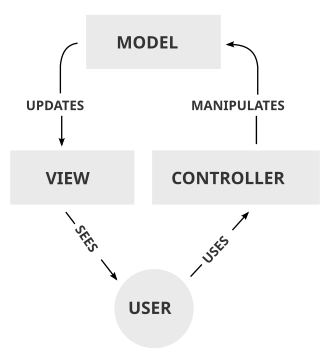
\includegraphics[width=0.9\textwidth]{architecture.png}
  \caption{System architecture diagram.}\label{fig:architecture}
\end{figure}

\subsection{Model Component}

The Model component manages the game's core data structures and business logic, organized into several modules:

\begin{itemize}
  \item \textbf{Game:} Central component that maintains the overall game state, including current game state, score, level progression, and timer management. The \texttt{Game} struct serves as the primary data container for all game entities.
  \item \textbf{Entity:} Defines the base \texttt{Entity} structure used for all game objects (player, enemies, bombs, walls, bricks). Provides common functionality such as position management, sprite handling, and movement.
  \item \textbf{Board:} Handles maze parsing from text files and maintains the spatial representation of the game maze. Manages different board elements and provides the foundation for collision detection.
  \item \textbf{Sprite:} Manages sprite creation from XPM files and animated sprites for dynamic entities. Handles sprite rendering and animation frame updates.
  \item \textbf{Resources:} Centralizes asset management by loading and storing all game sprites, ensuring efficient memory usage and providing a single access point for graphical resources.
\end{itemize}

\subsection{View Component}

The View component is responsible for all rendering operations and visual presentation:

\begin{itemize}
  \item \textbf{Rendering:} Implements frame caching to optimize performance, drawing different screens based on game state (start menu, pause menu, game screen, win/lose screens).
  \item \textbf{Game Visualization:} Renders the game board, all entities, user interface elements (score, lives, timer), and provides visual feedback for player interactions.
  \item \textbf{Menu System:} Handles drawing of interactive menus with mouse hover highlighting and button states.
\end{itemize}

\subsection{Controller Component}

The Controller component manages input handling and system-level operations:

\begin{itemize}
  \item \textbf{Device Drivers:} Low-level modules for timer, keyboard, mouse, graphics and RTC hardware, providing hardware abstraction.
  \item \textbf{Interrupt Handlers:} Coordinates all hardware interrupt subscriptions and delegates interrupt processing to appropriate handlers.
  \item \textbf{Input Module:} Abstracts keyboard input by converting scan codes into logical key representations (\texttt{KEY\_UP}, \texttt{KEY\_DOWN}, etc.) and defines interaction areas for menu navigation.
  \item \textbf{Event Handlers:} Processes high-level game events from keyboard, mouse, timer, and RTC interrupts. Translates raw input into meaningful game actions and state changes.
\end{itemize}

\subsection{Communication Patterns}

The MVC components communicate through the following interfaces:

\textbf{Controller $\rightarrow$ Model:} Hardware interrupts are processed by interrupt handlers, which call event handlers that modify the game state. For example, keyboard events trigger player movement by calling movement functions that update entity positions in the game model.

\textbf{Model $\rightarrow$ View:} The view component receives the current game state and renders the appropriate visual representation. The \texttt{draw\_next\_frame()} function determines which screen to display based on the game's current state.

\textbf{Main Loop:} The main game loop in \texttt{proj.c} orchestrates the entire system by receiving hardware interrupts, processing them through the controller, updating the model, and triggering view updates. This event-driven architecture ensures a clear separation of concerns.

The architecture's modularity allows for easy maintenance and extension, with each component handling its specific responsibilities while maintaining loose coupling through well-defined interfaces.

\section{Devices and Interfaces Used}

This project integrates five devices --- Timer, Keyboard, Mouse, Video Card (VBE/VGA) and the  Real-Time Clock (RTC) --- to handle timing, input, and rendering.

\subsection{Timer}

The Timer is set to 60 Hz to synchronize rendering and game updates. On each IRQ 0, \texttt{timer\_handler(game)} calls \texttt{timer\_int\_handler()} to increment a tick counter, then executes \texttt{draw\_next\_frame(game)} --- copying the static buffer into the back buffer, blitting all dynamic sprites, and calling \texttt{vbe\_flip\_page()} --- to render a new frame.

After rendering, \texttt{handle\_timer\_event(game, timer\_get\_counter())} updates animations (\texttt{player.update}, \texttt{enemy.update}) and processes timed logic (\texttt{update\_bombs()}, \texttt{update\_explosions()}) when \texttt{state == GAME}, ensuring fluid motion.

\subsection{Keyboard}

The PS/2 keyboard handles directional and command input. Each IRQ 1 reads a scancode via \texttt{get\_scancode()}, then \texttt{translate\_scancode()} maps it to a \texttt{Key} (arrows/WASD, Enter, Space, ESC). In START/PAUSE, arrow or A/D keys adjust \texttt{game->menu\_option}, Enter confirms, and ESC cancels or returns. In GAME, arrows/WASD call \texttt{move\_player()}, Enter/ESC pauses, and Space places a bomb behind the player based on \texttt{player.dir}.

\subsection{Mouse}

The PS/2 mouse provides menu navigation and bomb placement. Each IRQ 12 reads raw PS/2 packets (\texttt{mouse\_ih()}/\texttt{mouse\_sync()}) and decodes X/Y deltas and button states into a \texttt{mouse\_info\_t} struct. After parsing, we update the cursor's stored coordinates by adding those deltas. In START/PAUSE, the cursor's position is compared against predefined rectangular regions to set \texttt{game->menu\_option}, and a left-click confirms (start, resume, back, or exit). In GAME, a left-click maps the cursor to a grid cell and calls \texttt{drop\_bomb(game, x\_tile, y\_tile)} to place a bomb.

\subsection{Video Card (VBE/VGA)}

We initialize a linear VGA mode and employ triple buffering with page flipping to render all game entities' sprites without flicker.

The rendering process works as follows: each frame, \texttt{draw\_next\_frame(game)} first copies a cached static buffer (containing background and UI elements) into the current back buffer in VRAM, then uses \texttt{draw\_sprite()} to blit dynamic sprites (player, enemies, bombs, explosions, power-ups, cursor). Finally, \texttt{vbe\_flip\_page()} calls VBE function 0$\times$07 with sub-function 0$\times$80 (Set Display Start during Vertical Retrace) to change the display start to point to the completed buffer, then cycles \texttt{buff\_index} to the next buffer, ensuring smooth frame transitions without flickering.

\subsection{Real-Time Clock (RTC)}

The RTC is programmed to generate a 1 s periodic interrupt that drives enemy AI, the in-game level timer, and door timers. On each IRQ 8, \texttt{rtc\_handler(game)} clears the interrupt via \texttt{rtc\_ih()} and calls \texttt{handle\_rtc\_event(game)}.

If the game is in the GAME state, \texttt{handle\_rtc\_event()} advances each enemy one tile (\texttt{schedule\_enemy\_moves()}), decrements door open/close timers (\texttt{update\_door\_timer()}) and decrements the level timer (\texttt{update\_level\_timer()}).

\section{Differentiating Features}

\begin{itemize}
  \item \textbf{Triple Buffering with Frame Cache:}
    We draw menus and game boards once into a RAM-based cache. Each frame, we copy that cached image into the back buffer, overlay only dynamic sprites. This three-stage approach (cache → back buffer → VRAM) minimizes redundant drawing and tearing.

  \item \textbf{RTC-Driven Timing and AI:}
    By using a 1 Hz clock interrupt to move enemies and update door/level timers, we decouple these actions from the frame rate, making timed events run precisely in real time.

  \item \textbf{Fluid Sprite Animations:}
    Every moving entity maintains an \texttt{animation\_frame} index. During rendering, \texttt{draw\_sprite()} picks the correct XPM frame based on this index, resulting in smooth, frame-accurate animations.

  \item \textbf{Memory Efficiency with Minimal \texttt{malloc()} Usage:}
    All sprites, entities, and board data are allocated statically at startup. Aside from one-time allocations for the graphical resources, frame cache and back buffer, no \texttt{malloc()} calls occur during gameplay, reducing fragmentation and minimizing wasted memory.

  \item \textbf{Automatic, Extensible Levels:}
    Levels load from \texttt{level1.txt}, \texttt{level2.txt}, etc.; \texttt{load\_next\_level()} advances automatically (or sets WIN if no file), allowing easy addition of new maps and automatic level progression.
\end{itemize}


\section{Conclusion}
Summarize achievements, limitations, and possible future extensions. % TODO

\end{document}
